\documentclass[11pt,a4paper]{article}
    \usepackage[margin=2.5cm]{geometry}
    \usepackage{enumitem}
    \usepackage{hyperref}
    \usepackage{tikz}
    \usetikzlibrary{arrows.meta,positioning,shapes.geometric}
    \title{Teaching Administration Tools}
\author{Jordi Vill\`a-Freixa \texttt{<jordi.villa@uvic.cat>}}
    \date{\today}

    \tikzset{
      methodbox/.style={
        rounded corners=6pt,
        draw=blue!50!black,
        line width=0.9pt,
        fill=blue!6,
        minimum width=13cm,
        text width=11.8cm,
        align=left,
        inner sep=8pt
      }
    }

    \begin{document}
    \maketitle

    \section*{Scope}
    This folder currently focuses on automating repetitive teaching tasks from spreadsheet-like exports, especially individualized assessment material.

    \section*{Material in this folder}
    \begin{itemize}[leftmargin=*]
\item \texttt{Individualized\_tests\_from\_Moodle\_csv.ipynb}
    \end{itemize}

    \section*{Method summary}
    \begin{itemize}[leftmargin=*]
\item \textbf{CSV-based test customization}. The notebook reads Moodle-style participant and question data and builds individualized outputs for each student.
\item \textbf{Template-based file generation}. The workflow combines tabular inputs with text templates to emit per-student files and linkage tables.
\item \textbf{Lightweight course administration automation}. The examples emphasize practical scripting for recurring teaching duties rather than full LMS integration.
    \end{itemize}

    \section*{Method scheme}
    Figure~\ref{fig:summary} is drawn directly in LaTeX with TikZ. It is a compact conceptual map of the main workflows discussed in this folder.

    \begin{figure}[ht]
    \centering
    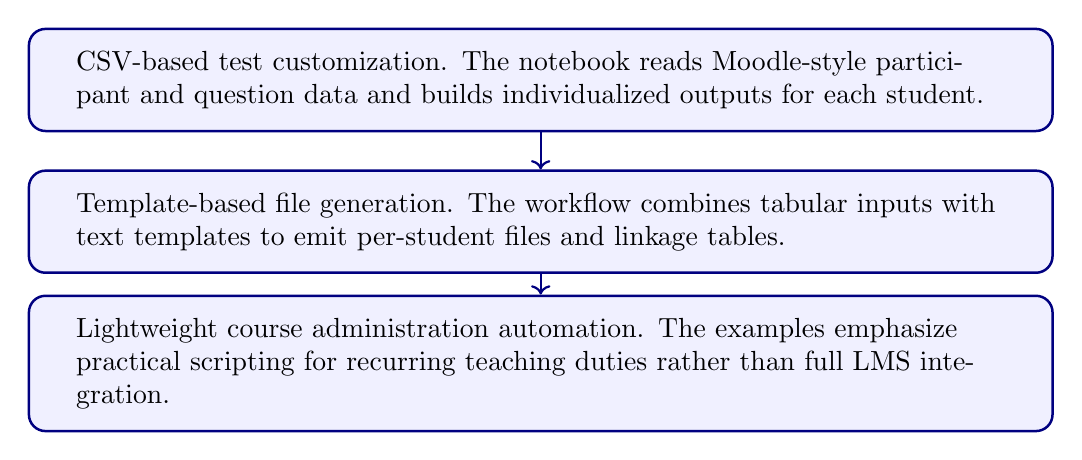
\begin{tikzpicture}[x=1cm,y=1cm]
    \node[methodbox] (m0) at (0,0.0) {CSV-based test customization. The notebook reads Moodle-style participant and question data and builds individualized outputs for each student.};
    \node[methodbox] (m1) at (0,-1.8) {Template-based file generation. The workflow combines tabular inputs with text templates to emit per-student files and linkage tables.};
    \node[methodbox] (m2) at (0,-3.6) {Lightweight course administration automation. The examples emphasize practical scripting for recurring teaching duties rather than full LMS integration.};
    \draw[->, thick, color=blue!50!black] (m0.south) -- (m1.north);
    \draw[->, thick, color=blue!50!black] (m1.south) -- (m2.north);
    \end{tikzpicture}
    \caption{Conceptual scheme for the methods in the teachingTools folder.}
    \label{fig:summary}
    \end{figure}

    
\bibliographystyle{plain}
\bibliography{../references}

\section*{Disclaimer}
These documents were generated with the assistance of ChatGPT 5.4. The material has been reviewed by the author before inclusion in this repository, but it is not free from possible errors.

\end{document}